%!TEX root = proj_report_outline.tex
\chapter{Implementation}\label{C:webApplicationImplementation}

\section{Implementation Details}
The standard web application functionality required within the prototype, such as authentication, request life-cycles and password resets, was straightforward as Ruby on Rails solves many of these problems, and offers a wealth of libraries that can assist. The Pitch Card functionality and scope of disclosure functionality described in the Sections \ref{C:requirements} and \ref{C:design_web} were implemented from the ground up. In this Section these two functionality item's implementation details are explored.

\subsection{Pitch Card System}
As exemplified in Section \ref{C:requirements} Callaghan Innovation's specification for how the Pitch Card system works was quite mature and detailed. At it's core it required that users be able to initiate Pitch Cards and browse Pitch Cards, with the further ability to contribute suggestions or comments. To do this the web application separates the action's responsibilities. As discussed in Section \ref{SS:frameworkSelection} Ruby on Rails is architected on the MVC architecture pattern. Following Ruby on Rails convention the PitchHub prototype has models, views and controllers for each resource. The controllers adhere to the RESTful design principles, where resources are accessed using conventional HTTP resource methods and relationships are expressed via resource-nesting. The models, as designed in Figure \ref{fig:class_diagram}, were implemented with the Mongoid \cite{Mongo4:online} Object Document Mapper (ODM) for MongoDB. The Mongoid ODM subscribes to the ``convention over configuration'' philosophy that is held highly in the Ruby on Rails framework, offering a simple façade over the MongoDB query language. The views were implemented with HTML, SASS (CSS), and JavaScript. To enhance the user experience AJAX was implemented to speed up page load times by loading secondary or non-essential data asynchronously. AJAX was also heavily used in user interactions, such as contributing a suggestion/comment and setting disclosure scopes (as an initiator).
\par
Figure \ref{fig:pitch_card_pitchhub} showcases the prototype's Pitch Card view from the initiator's perspective. The view can be deconstructed as follows: the sidebar contains the links to the main pages, the navigation bar contains the search box and user management drop-down, the main page space contains the Pitch Card and it's associated suggestions. Figure \ref{fig:dashboard_pitchhub} contains the same sidebar and navigation bar however the main page space contains a grid of mini-pitch card views consisting of the Pitch Card's image (if any) as well as the \textit{Value Proposition} pitch point.

\subsection{Scope of Disclosure}
As previously discussed in Section \ref{S:systemModel} and shown in Figure \ref{fig:class_diagram} the scope of disclosure functionality is implemented on both Pitch Card and Suggestion/Comment models. For Pitch Cards this scope of disclosure is achieved through a combined effort at the database level and at the application level. To illustrate this consider the \ref{fig:dashboard_pitchhub}. When the user loads up the dashboard the database is queried asking for Pitch Cards that the current user is able to see (if any). How this first step works is through the use of MongoDB's aggregation pipeline \cite{Aggre7:online}. The aggregation pipeline in this instance deals with the fact that users assume different roles in the context of different Pitch Cards, and Pitch Cards themselves are heterogeneous in the scopes they are defined with. Unlike role-based Access Control Lists, where a user is checked if their role satisfies a particular permission level, the pipeline designed for PitchHub checks the user against each role of the Pitch Card and then against the Pitch Card's visibility scope. This single pipeline aggregation query basically checks a matrix of constraints to check each context. This is visualised in Figure \ref{fig:pipeline}.

\begin{figure}[ht]
    \centering
    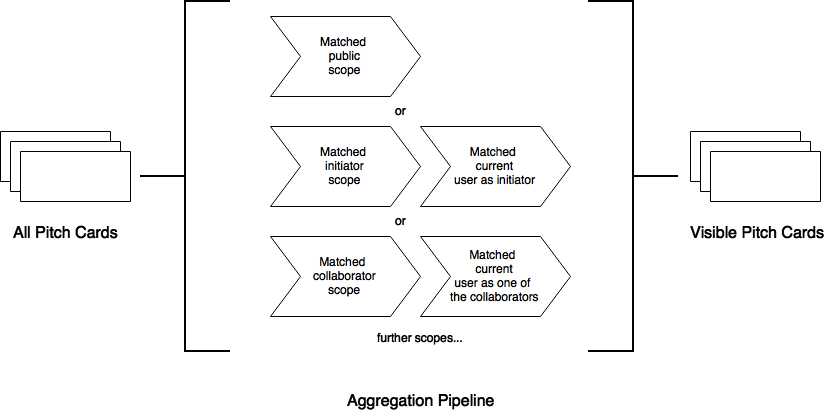
\includegraphics[width=1\textwidth]{pipeline}
    \caption{The pipeline aggregation query used to find all visible Pitch Cards checks for the scoping of the Pitch Card from the context of the current user.}
    \label{fig:pipeline}
\end{figure}

Continuing the example above, once the viewable Pitch Cards for the Dashboard view have been retrieved from the database the application applies the identity scopes for each Pitch Card in the view. This piece of functionality decides whether the the initiator will appear by their name or by `anonymous'. The way this is implemented is made simple through the ODM, where when the Pitch Card object is retrieved, the Pitch Card's nested scope objects are also retrieved. As seen in Figure \ref{fig:class_diagram} these scope objects implement the strategy pattern, so when they are retrieved the application is able to easily check whether the current user is authorised to see the Pitch Card's author agnostic of the actual scope being used. The use of the strategy pattern removes the need to do the less-pragmatic and less-extensible type-checking on scope objects to determine what scoping business logic should be used.
\par
The marriage of database-level and application-level scoping caters to the context of the request's life-cycle stage to maximise efficiency. Certainly, it would have been possible to use the strategy pattern object scoping instead of what is essentially type-checking in the aggregation pipeline query to achieve this scoping. However, at this point in the request the application does not have Pitch Card objects (and their nested scope objects) to scope by, therefore by expressing this logic in the database query the application is able to appropriately apply scope given the context, retrieving only the viewable Pitch Cards.

\section{Implementation Challenges}

\subsection{Virtualised Environment}
The time-constrained weekly/bi-weekly meetings with Callaghan Innovation elicited the need for their own locally hosted PitchHub instances. Their own PitchHub instances enabled them to check the progress of the prototype, answer UI/UX questions, and show the prototype to other Callaghan Innovation personnel. 
\par
Personally configuring the environment and setting up PitchHub was an option, however this would have still been a lengthy process detracting from actual meeting. Furthermore it would have been infeasible to repeat this for each stakeholder and their various machines. Requiring the stakeholders to do this themselves would have similarly been infeasible as configuring a locally hosted Ruby on Rails application is a non-trivial task \cite{Roma:personalCommunications}, to exemplify this StackOverflow has excess of 50,000 questions in relation to Ruby on Rails installation/configuration \cite{StackOverflowProblem1:online, StackOverflowProblem2:online, StackOverflowProblem3:online, StackOverflowProblem4:online}.
\par
To solve this problem the PitchHub environment and installation process was automated using a combination of Chef and Vagrant scripts. Vagrant was employed to automate the Ubuntu virtual machine setup and Chef was leveraged to manage PitchHub's various environment dependencies (Ruby, a JS runtime, and MongoDB). By having this infrastructure/configuration implemented via code it also serves as documentation for the PitchHub environment and enables the use of version control within this aspect of the project. This process has the further advantage in that any future contributors to the project will have a very low barrier to entry in terms of setting up their own locally hosted PitchHub instance.

\subsection{Deployment}
As discussed in Section \ref{S:projectObjectives} one of the objectives was to have a prototype deployed for internal use by Callaghan Innovation. The deployment process of PitchHub consisted of two steps: first, setting up the infrastructure for the deployment and second, deploying the Ruby on Rails prototype onto the infrastructure. To support the first step, Callaghan Innovation provided a machine, racked it in their server room, and also configured the machine's domain name. I then completed the infrastructure setup by configuring the nginx HTTP server \cite{nginx2:online}, the Phusion Passenger application server \cite{phusionPassenger:online} and SSL. In regards to step 2, there exist a few prominent methods of deploying Ruby on Rails applications:
\begin{itemize}
    \item A manual process using a combination of SFTP and SSH, to transfer files and update environment variables.
    \item An automated process facilitated by Capistrano, a Ruby on Rails deployment library.
\end{itemize}

The manual process, while easier for the initial deployment, was decided against as the process is brittle in that it relies on the deployer to fulfil each deployment step correctly and in order. For a Ruby on Rails application this process at the very minimum consists of: transferring the updated application code, pre-compiling the assets, downloading any newly added libraries and updating the binaries. Should this be done incorrectly or in the wrong environment this manual process has no `undo' action, therefore the process of reverting the application must also be done manually. Capistrano alleviates these problems but at the cost of a steep-learning curve. Capistrano is similar to Vagrant in that the process is automated by scripts which automate the entire process. Ultimately, the initial investment in defining the scripts is negligible in comparison to the long term gains of robust and consistent deployments. PitchHub is currently hosted at \textit{pitchhub.net}, note that the current release is being used internally in Callaghan Innovation and requires an access code to sign up.

\begin{sidewaysfigure}[ht]
    \centering
    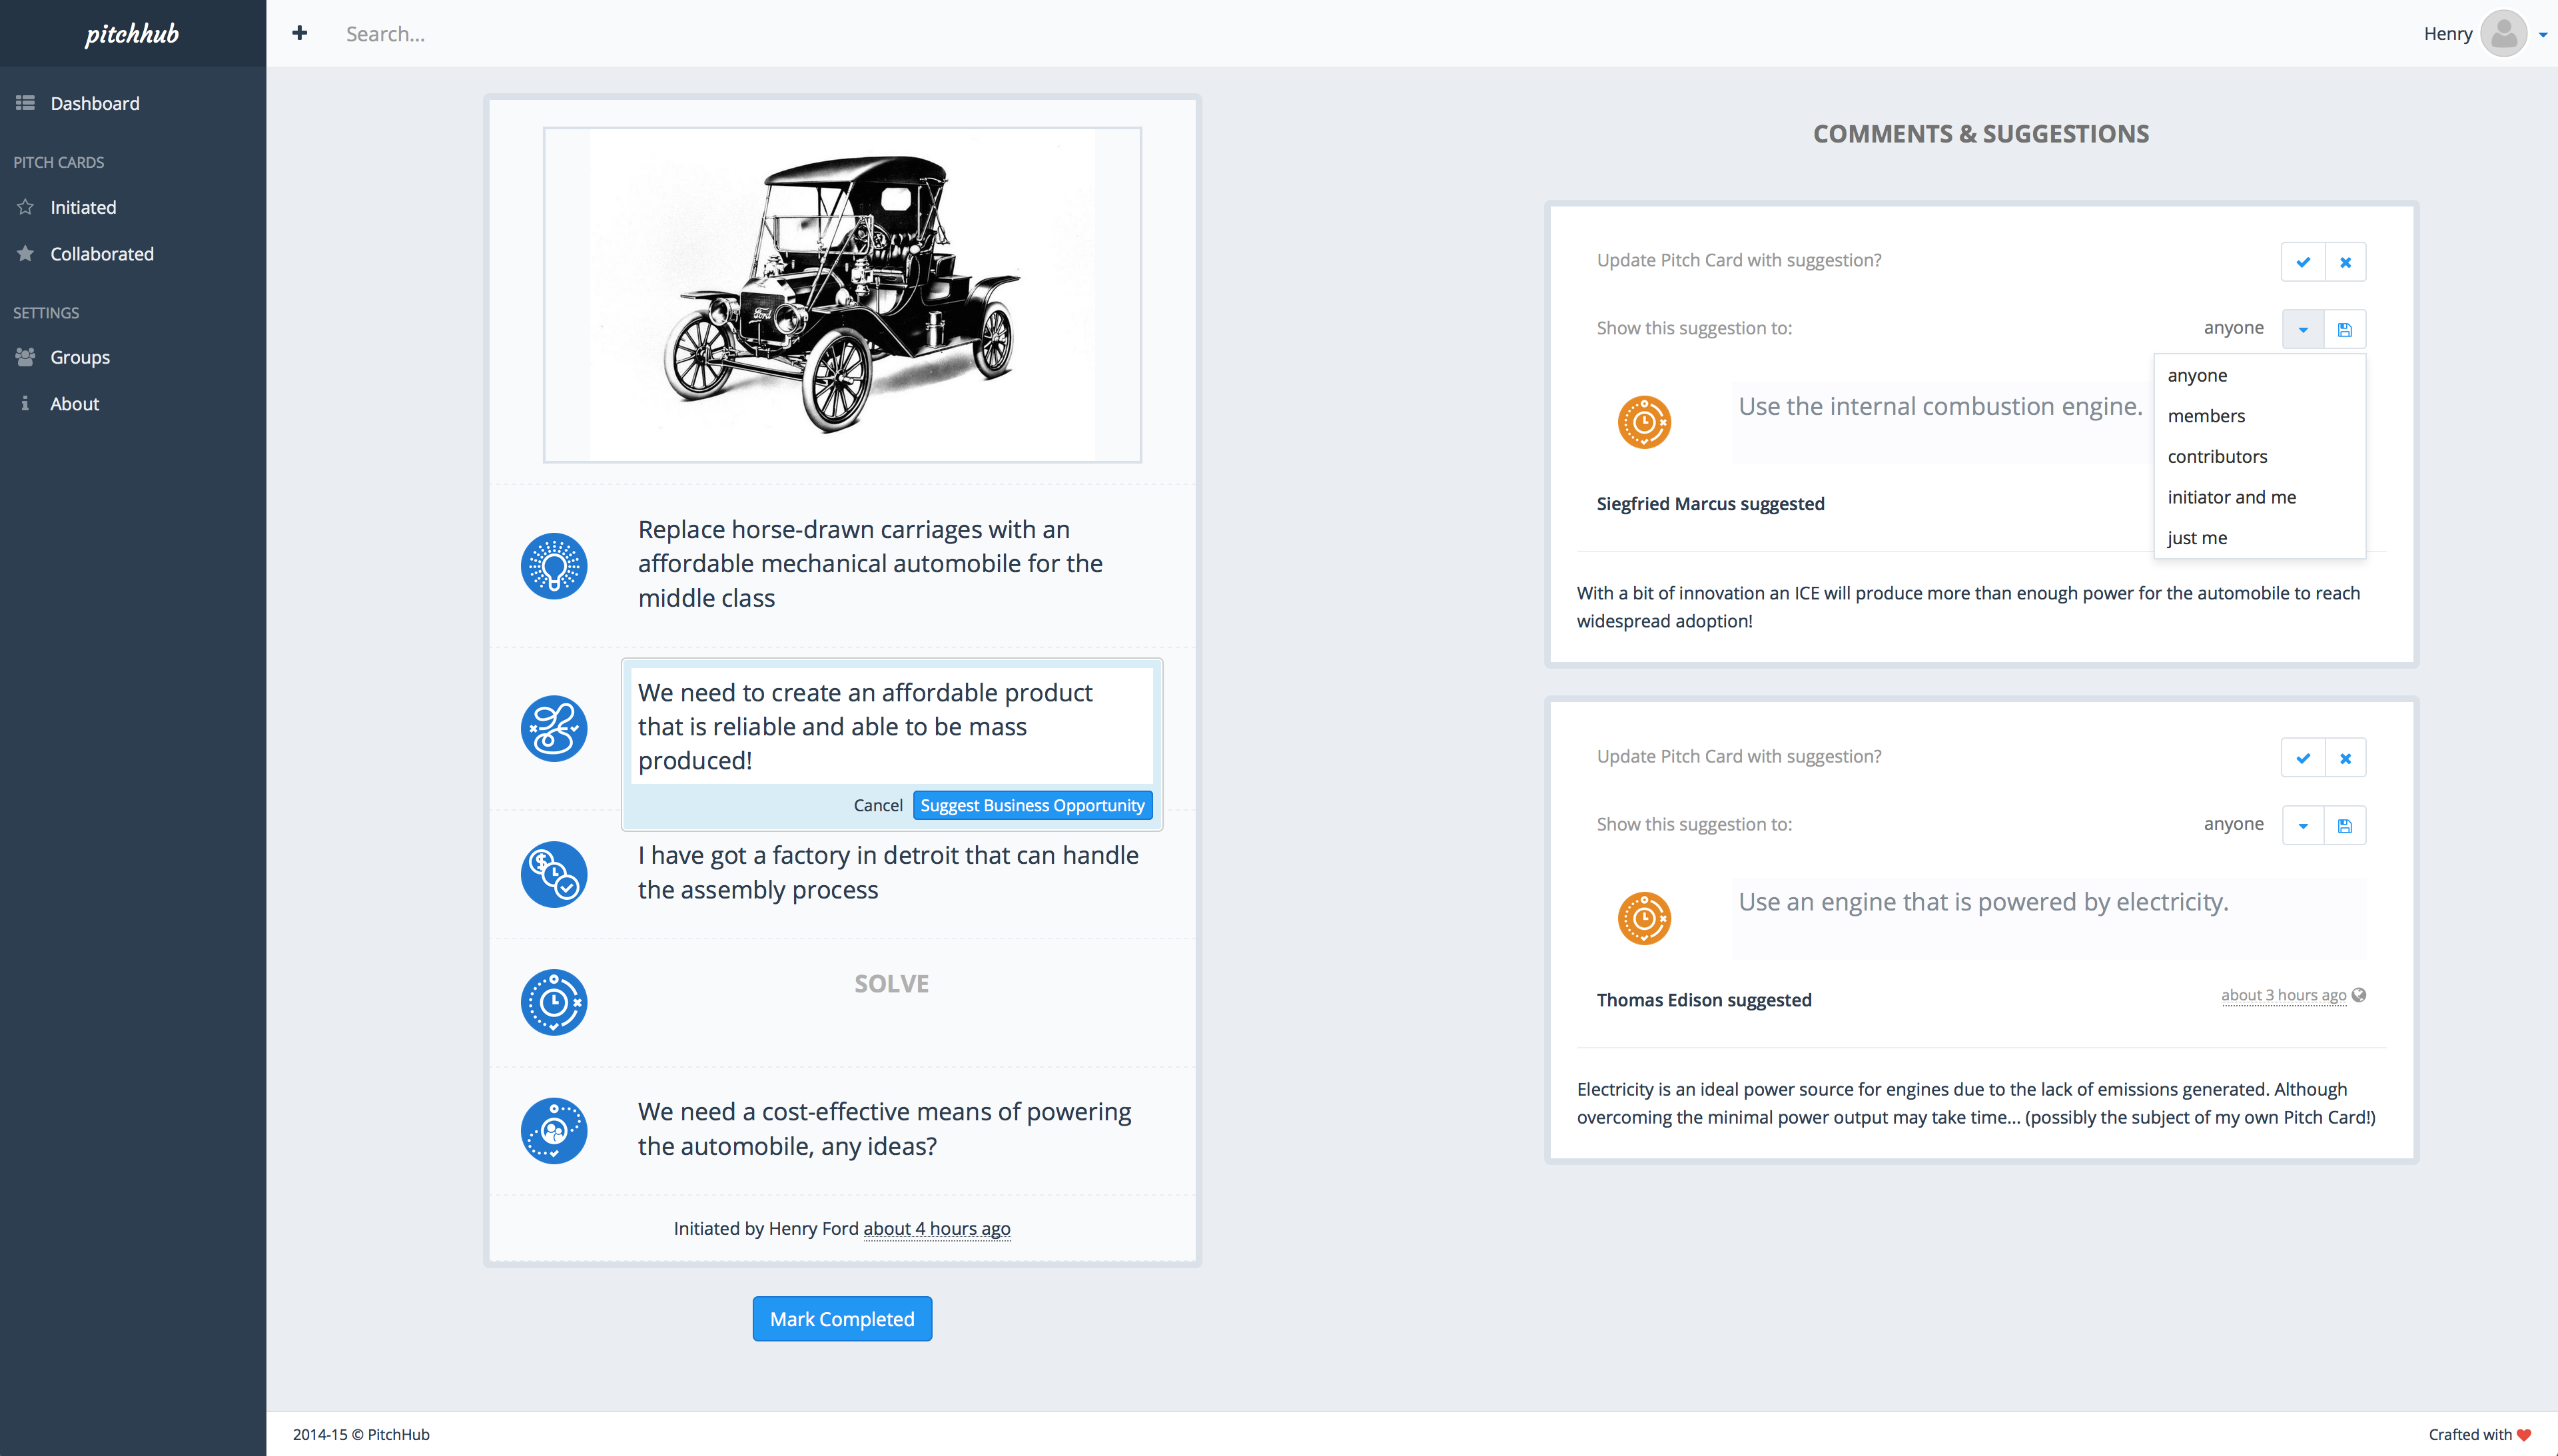
\includegraphics[width=1\textwidth]{pitch_card_pitchhub}
    \caption{Fictional Ford Model T Pitch Card view from the initiator's perspective. The view is divided into two sections the Pitch Card and it's suggestions/comments. In the Pitch Card half users perform in-line editing on a Pitch Point to make a suggestion. In the suggestion/comments half the initiator may accept or decline the suggestion and set the suggestion/comment's scope.}
    \label{fig:pitch_card_pitchhub}
\end{sidewaysfigure}

\begin{sidewaysfigure}[ht]
    \centering
    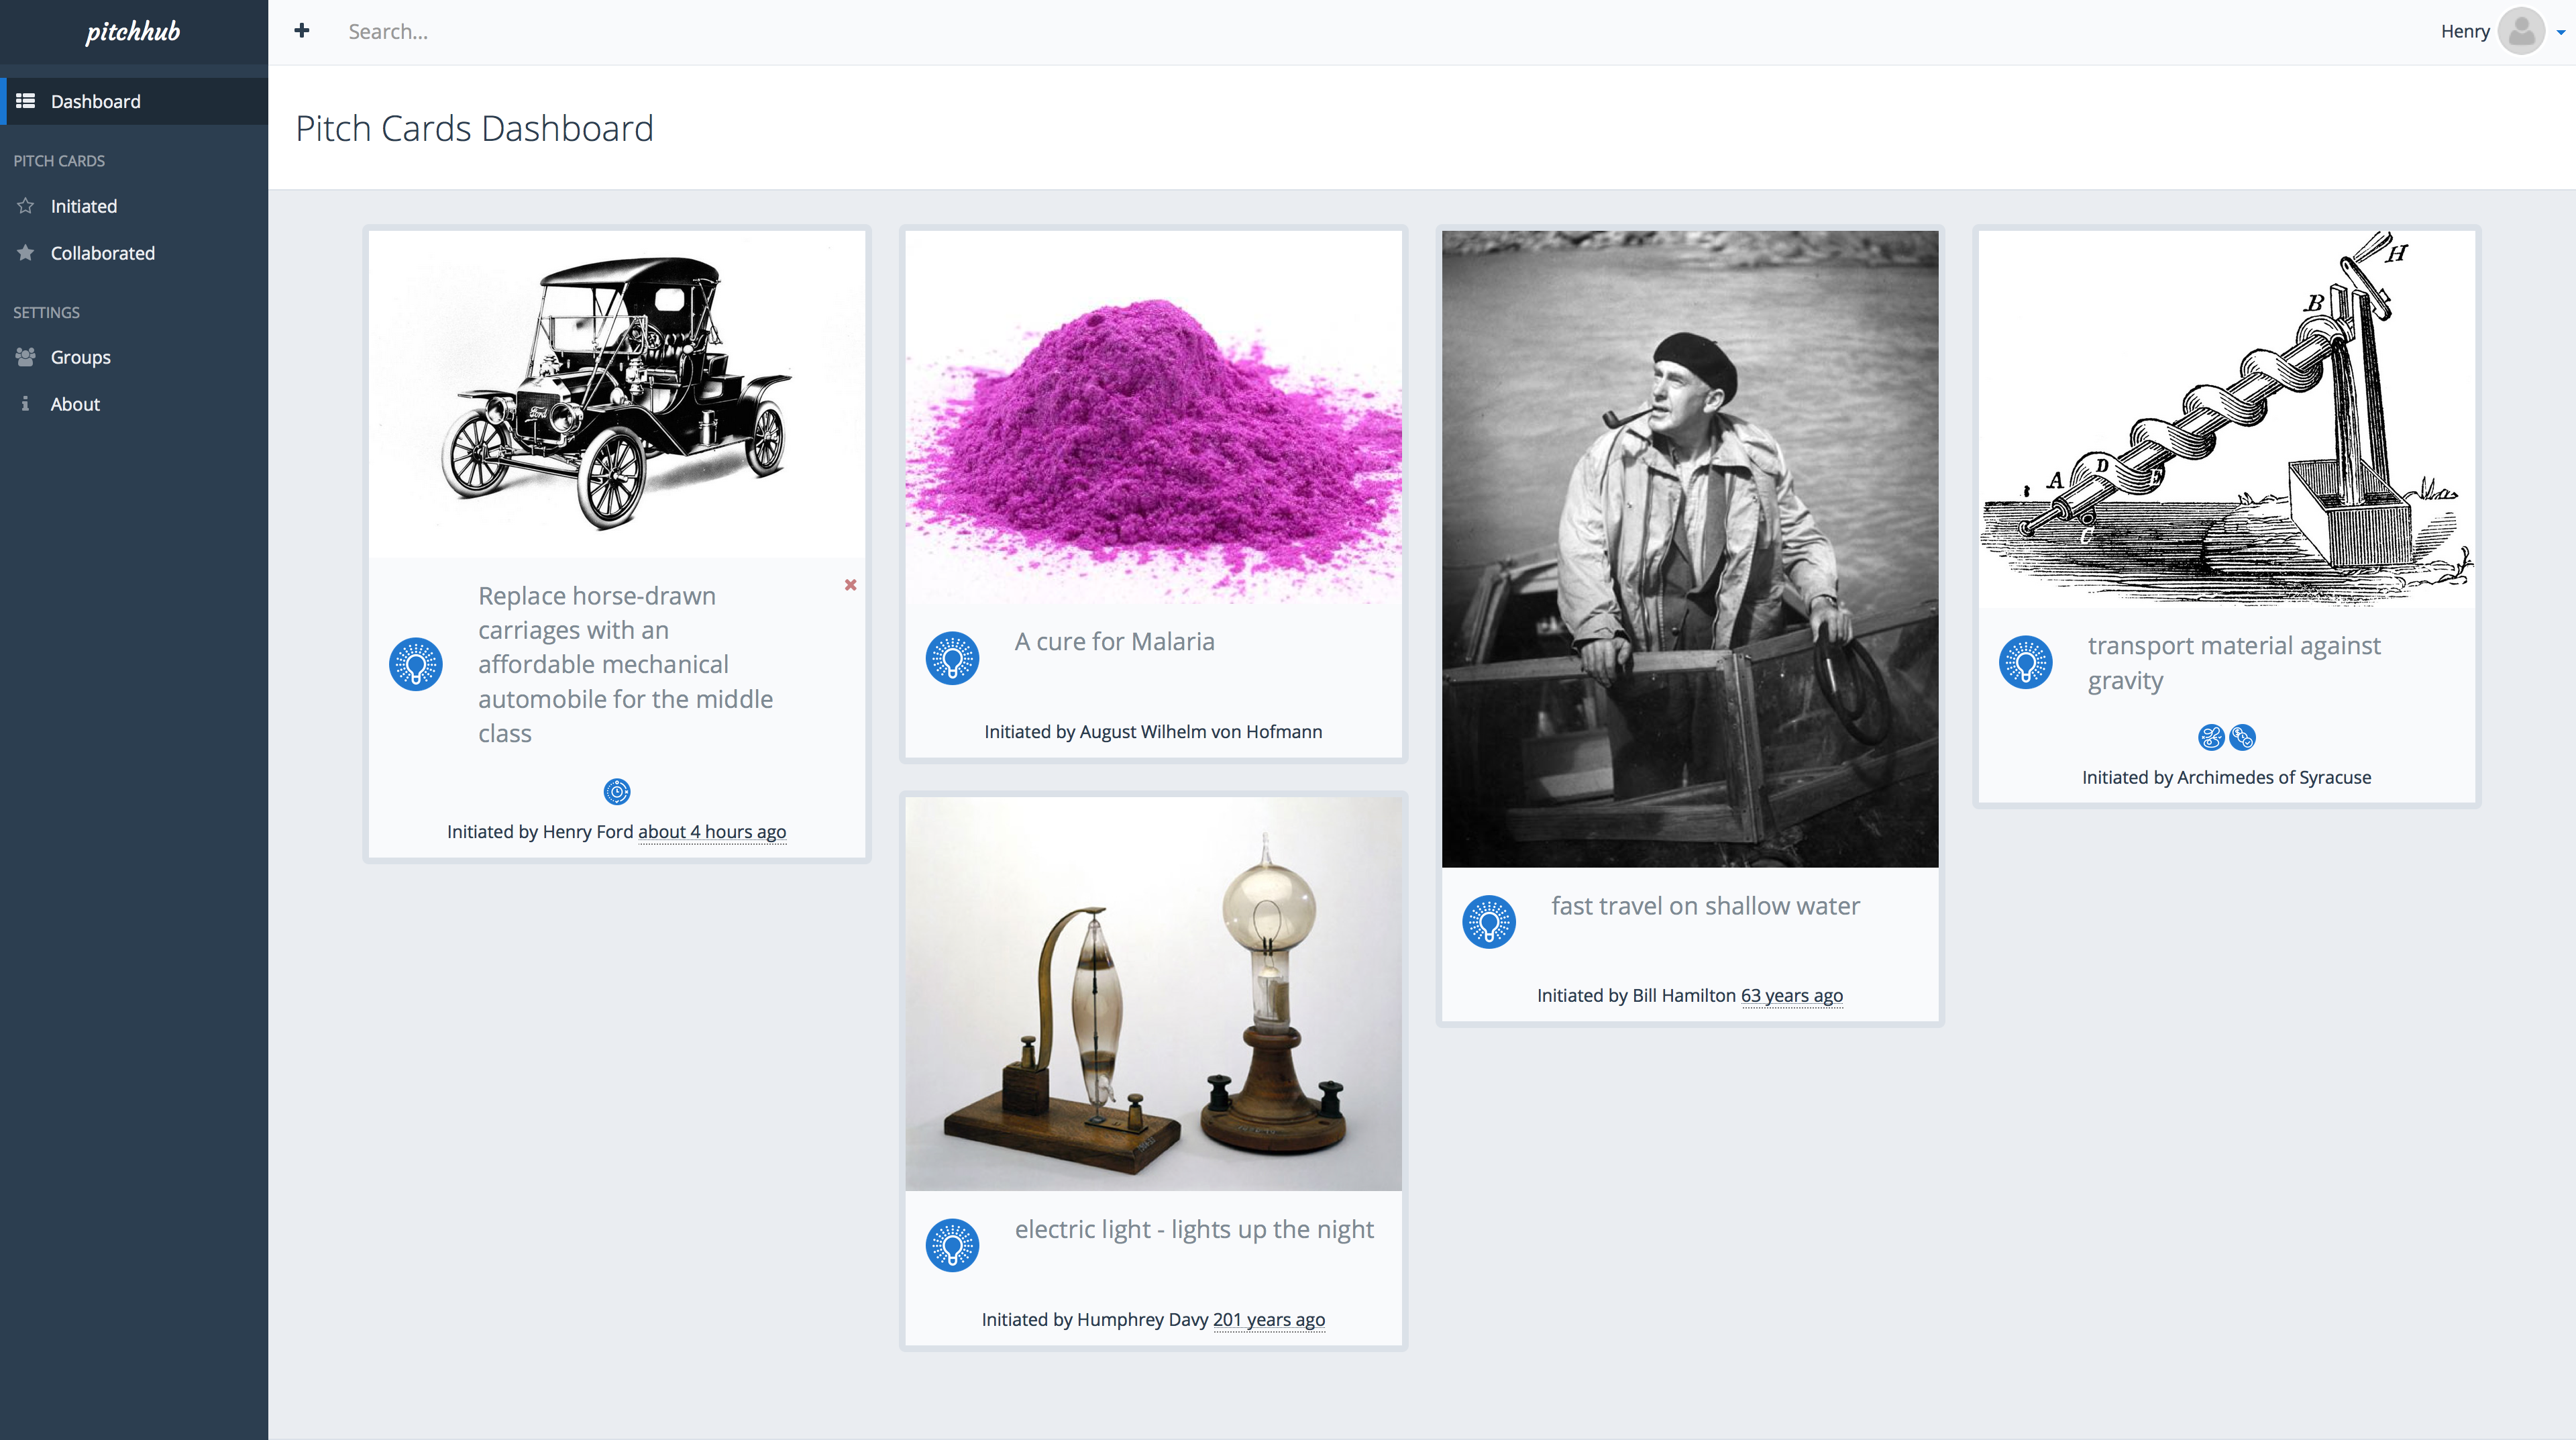
\includegraphics[width=1\textwidth]{dashboard_pitchhub}
    \caption{PitchHub's dashboard populated with fictional Pitch Cards. The grid layout displayed is responsive, so the Pitch Cards will reorganise and size to fit the user's device screen.}
    \label{fig:dashboard_pitchhub}
\end{sidewaysfigure}